\documentclass{article}

\usepackage{hyperref}

\usepackage{graphicx}
\usepackage{multimedia}
\usepackage{amssymb}

%\usepackage{algorithmic}
\usepackage{fancybox}
\usepackage{pseudocode}

\usepackage{pifont}
\usepackage{multirow}
\usepackage{slashbox}
\usepackage{pdfpages}
\usepackage{picture}

\usepackage{appendix}

\title{CS566 Parallel Processing \\ Assignment 04 \\ The Travelling Salesman Problem} 
\author{Camillo Lugaresi and Cosmin Stroe \vspace{20pt} \\ Department
of Computer Science \\ University of Illinois at Chicago}

\date{December 5, 2011}

\begin{document}

\maketitle
\newpage

For our assignment, we implemented a depth first search (DFS) based solution for
the travelling salesman problem (TSP), using the branch and bound optimization
to keep a global shortest cycle cost and to prune the search tree of paths which
cannot be optimal.  This ensures that our algorithm will exaust the search space and 
that the solution it finds is the most optimal one, while not wasting execution time by 
checking suboptimal paths.

\section{Algorithm Details and Formulations}

\subsection{TSPLIB95}

As inputs to our program we used the datasets part of the TSPLIB95, which is a
collection of TSP problems in an easy to read format.  We only used symmetric
TSP problems, as those are more challenging than asymmetric TSP problems.  Also,
the problems in TSPLIB95 have solutions which are published on the
website\footnote{\url{http://comopt.ifi.uni-heidelberg.de/software/TSPLIB95/}},
making it easy to check the correctness of our algorithms.

As part of our work, we implemented a parser for the TSPLIB95 datafiles which
reads the TSP datafile and produces a distance matrix.  The matrix is then used
for looking up the distances between nodes, as needed by our algorithm.

\subsection{Depth First Search: Branch and Bound}

The solution space of the TSP problem with $n$ nodes can be represented as a
tree of depth $d = n$.  At each node in the tree, there are $n - d$ possible
choices for branching, and each one must be explored or pruned.  A DFS traversal
of the tree starting from the root of the tree is necessary since the cycle cost
can only be recorded once the algorithm reaches a leaf node.   When reaching a
leaf node, we record the cost of the cycle if it is lower than our current
lowest cycle cost.

We then backtrack to the parent node and choose the next possible node and
search that branch; but we do this only if the cumulative cost of the current
path from root to the current node is less than the lowest cycle cost. 
Otherwise we abandon (prune) this branch, as we know we will not be able to
obtain an optimal cycle from this branch.

In our algorithm, we do not maintain the tree in memory; we only keep track of
the current path from root, as this is all the information we require when
running our algorithm.  We also keep track of the last visited node at every
level.  The last visited node is updated when work is given away to other
processors, so that the current processor will not explore a branch which has
been assigned to another computer.  Using the current path from root, and the
last visited node at every level, we can compute which node to visit next.

Each processor in our algorithm is given a search space which to exaust. At the
beginning, only node 0 has work, and the other processors must ask node 0 for
work.  When work is given away, that branch is marked as visited on the current
computer so that it is not traversed and also that it is not given away as work
to another requester.  When a cycle is found that is shorter than the global
shortest cycle, the new cost is broadcast to all the processors in the cluster,
so that they better prune their search spaces.

\subsection{Load Balancing: Asynchronous Round Robin}

As processors exaust the search space assigned to them, they must ask for work
to processors which are still working traversing their search space.  For the
purpose of load balancing, we use the asynchronous round robin method of keeping
a variable on our every processor with its next work partner from which to
request work.  Once a work partner is asked for work, the variable is
incremented to the next computer in a round robin fashion.  This is done
asynchronously for each processor, so the drawback to this approach is that
multiple processors can be asking for work to the same exact processors, however
because we need to traverse the entire space this does not affect our algorithm.

\subsection{Asynchronous MPI Messages}

All of our communication, except for receiving work, is done asynchronously. 
This is required because the processors cannot be synchronized in the servicing
of their messages, and synchronous messages would result in idle time. 
Receiving work is synchronous because after the work request is sent, we have
nothing to do but to wait for the answer of the work request.  All of the
message types we pass, shown in table \ref{tab:msg_tags}, are tagged so that we me
identify what type of message it is and invoke the correct message processing
function.


\begin{table}
	\centering
	\begin{tabular}{|c|c|p{4cm}|}
	\hline
	{\small Message Type} 			& {\small MPI Tag}								& \multicolumn{1}{|c|}{Description} \\ \hline
	{\small Upper Bound Broadcast}	& {\small \texttt{UB\_TAG (1)}}					& {\small Broadcast the new global shortest cycle path.} \\ \hline
	{\small Work Request}			& {\small \texttt{WORK\_REQ\_TAG (2)}}			& {\small Request work.} \\ \hline
	{\small Work Acknowledgement}	& {\small \texttt{WORK\_ACQ\_TAG (3)}}			& {\small Respond to a work request, either deny or a path describing the branch to be explored.} \\ \hline
	{\small Token}					& {\small \texttt{TOKEN\_TAG (4)}}				& {\small Pass the token used in termination detection.} \\ \hline
	{\small Termination Signal}		& {\small \texttt{TERMINATION\_TAG (5)}}		& {\small Passed when termination is detected.} \\ \hline
	{\small Best Path Request}		& {\small \texttt{BEST\_PATH\_TAG (6)}}			& {\small Reply to a best path request with the path of the best cycle.} \\ \hline
	{\small Best Path Transmit}		& {\small \texttt{BEST\_PATH\_REQ\_TAG (7)}}	& {\small Request the path of the best cycle stored on a processor.} \\ \hline
	
	
	\end{tabular}
	\caption{The message types and their tags handled in our communication.}
	\label{tab:msg_tags}
\end{table}

Once termination has been detected by the root processor (described in section \ref{sec:term_detect}), a best path request
is sent to the processor that broadcast the last upper bound in order to receive the actual path of the 
best cycle.  When the root processor received the best path, it sends a termination signal message to all other processors
in the cluster and exits the program.  Upon receiving the termination signal, the processors service their pending messages
and exit the program.

\subsection{Termination Detection}
\label{sec:term_detect}

For termination detection we use Djikstra's Token Termination Detection algorithm. 
In order to simplify our message handing code, the token termination detection is only
initiated by the root node.  All the other processors pass on the token but will not 
initiate a token request.  Instead, they wait for a termination message which is sent 
from the root processor upon a successful termination detection.

% \begin{figure}
% 	\centering
% 	\includegraphics[width=1.0\textwidth]{images/cannon-skew.pdf}
%     \label{fig:cannon-skew}
%     \caption{Explanation of the skew operation in Cannon's algorithm.}
% \end{figure}


\section{Input and parameters}

We ran our experiments using problems of sizes $n = \{ 14, 17, 21, 24 \}$,
namely burma14, gr17, gr21, and gr24.  For our processor size we consider the total number 
of threads running, not differentiating between processors or cores.  This is because
communication is not a bottleneck in this algorithm and we can take full advantage of every core
on a computer.

\section{Results}

\begin{table}
	\centering
	\begin{tabular}{|c|c|c|c|c|}
	\hline
	Num. threads & burma14 	& gr17 	& gr21 	& gr24 \\ \hline
	1			 &			&		& 		&		\\ \hline
	4			 &			&		&		&		\\ \hline
	8			 &			& 		& 		& 		\\ \hline
	16			 & 			& 		& 		& 		\\ \hline
	\end{tabular}
\end{table}

\section{Analysis and Lessons}

\clearpage

\appendix
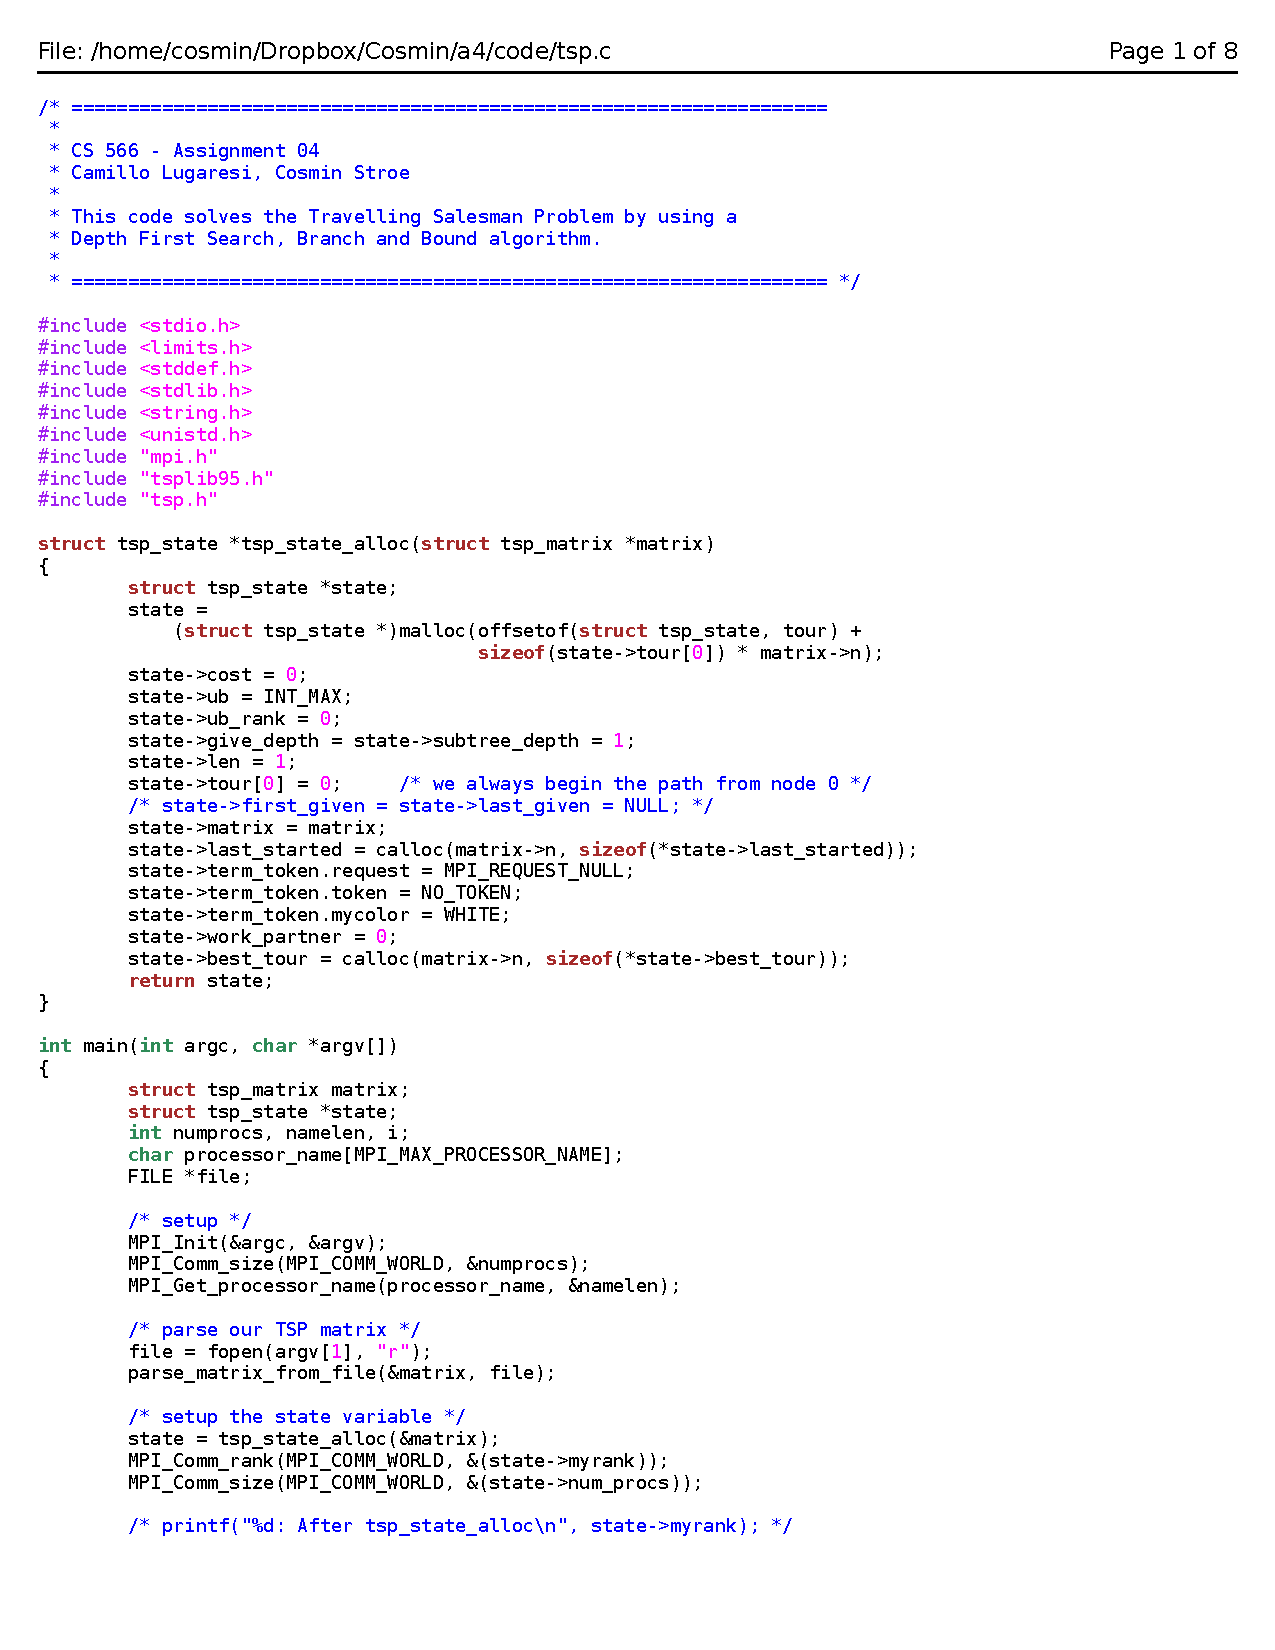
\includepdf[pages=-]{code/tsp_c.pdf}
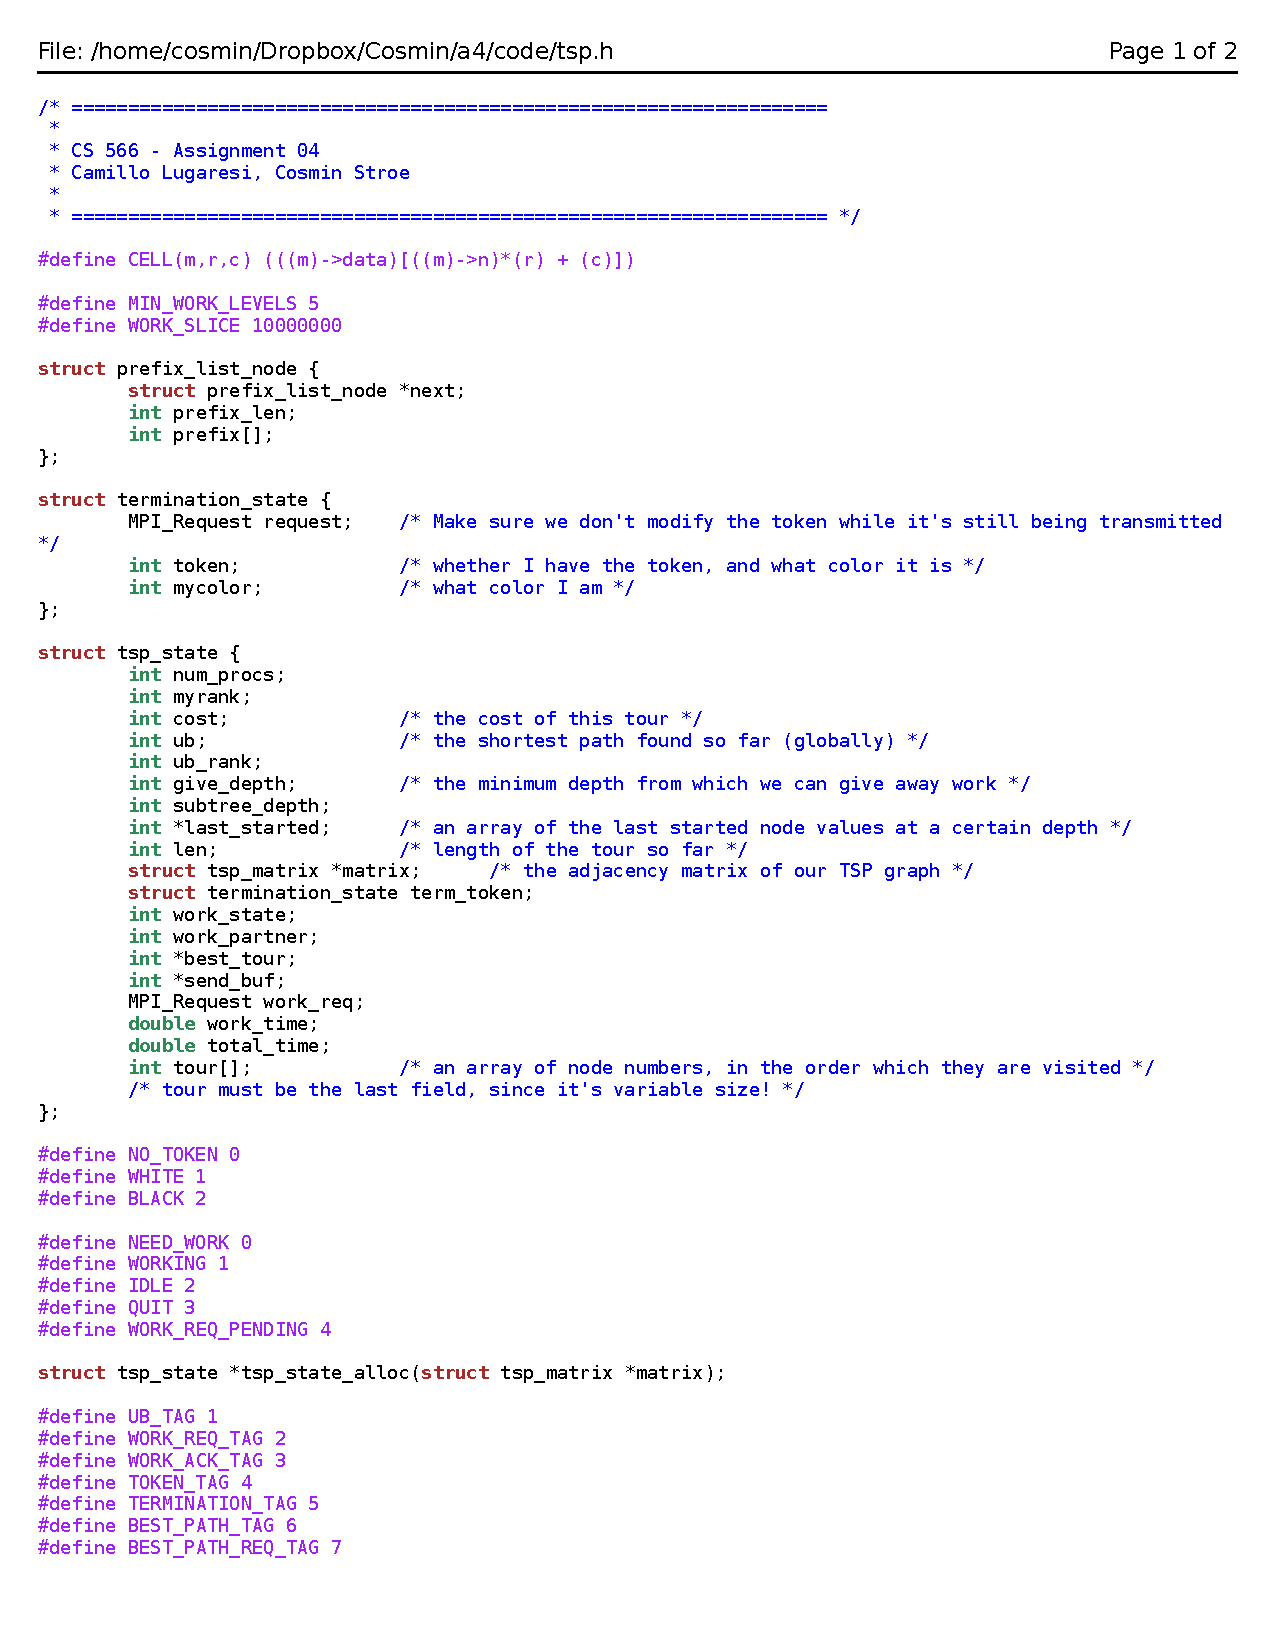
\includepdf[pages=-]{code/tsp_h.pdf}
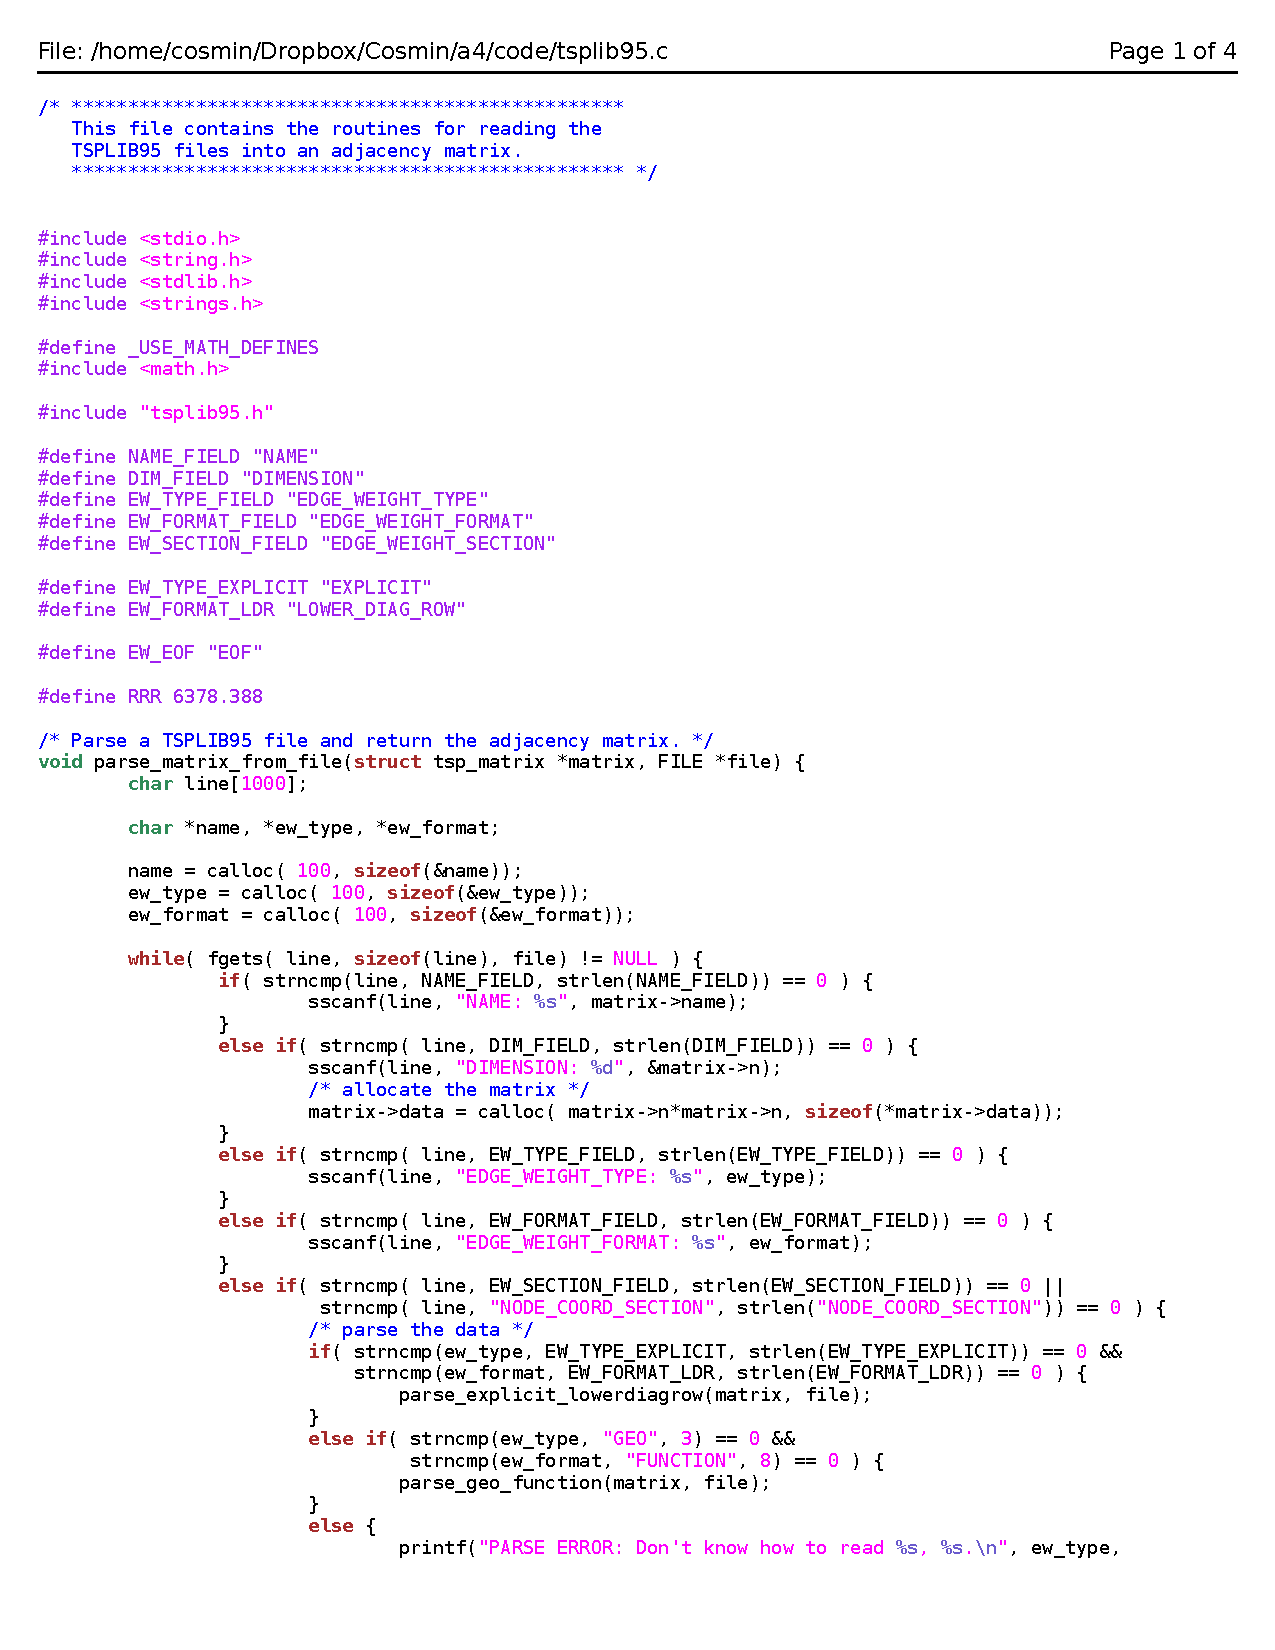
\includepdf[pages=-]{code/tsplib95_c.pdf}
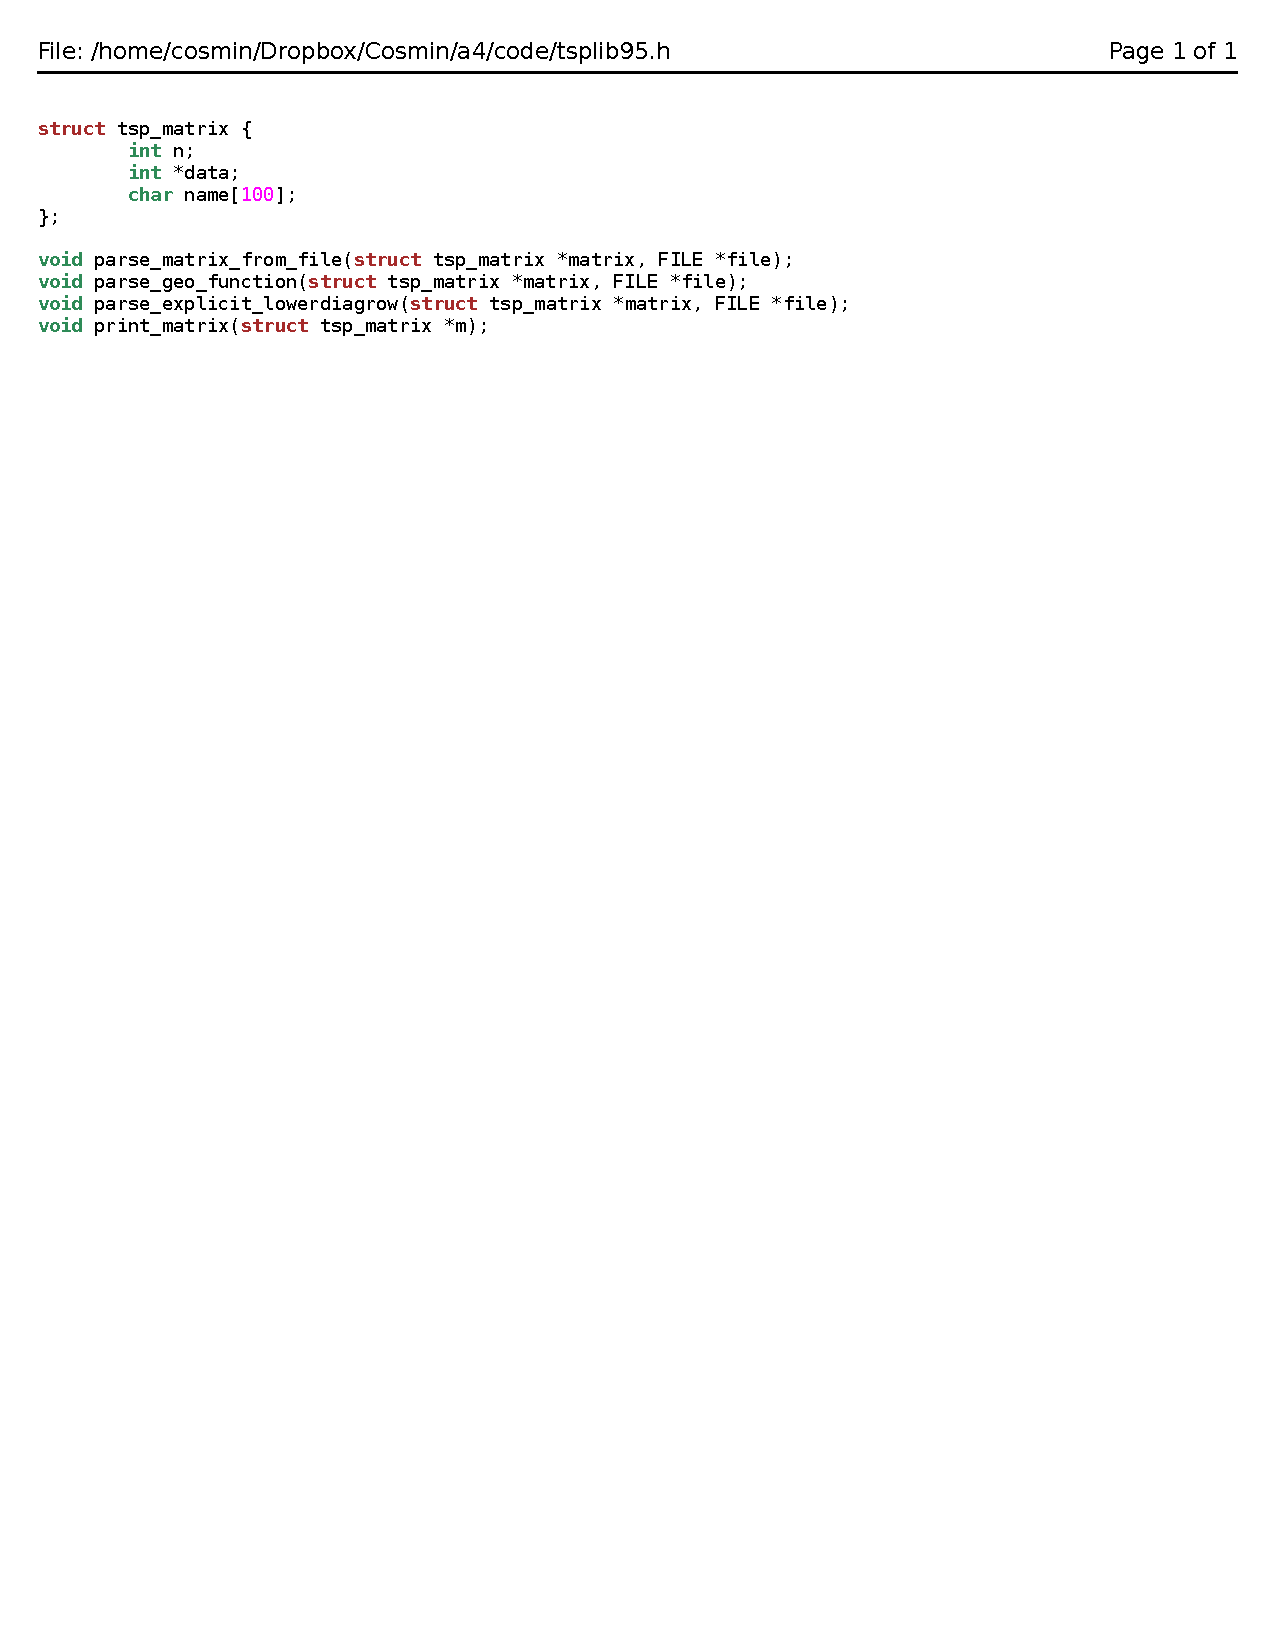
\includepdf[pages=-]{code/tsplib95_h.pdf}
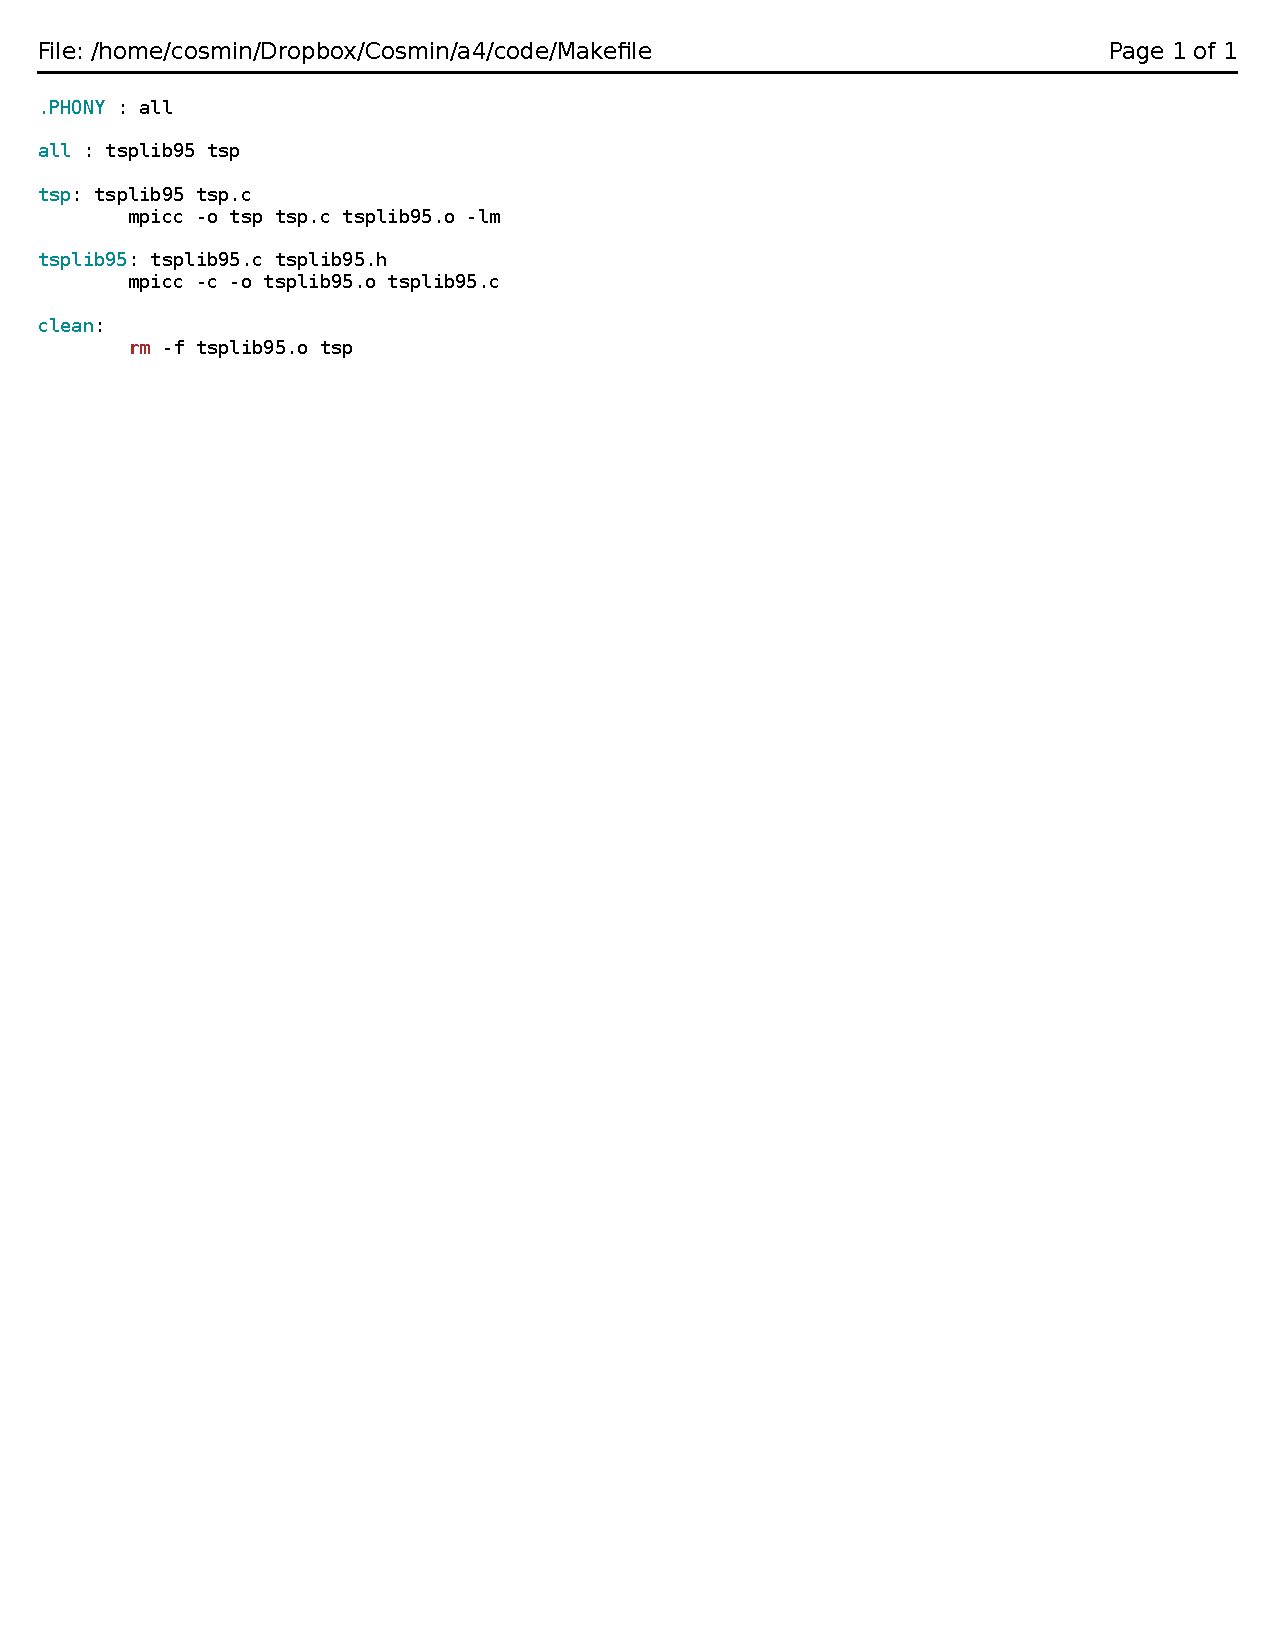
\includepdf[pages=-]{code/Makefile.pdf}

\end{document}
